In next-to-leading order a new production mechanism enters that is induced by a light quark, so we have to consider the process
\begin{equation}
\Pggx(q) + \Pq(k_1) \rightarrow \PQ(p_1)+\PaQ(p_2) + \Pq(k_2)
\end{equation}
where all contributing diagrams are depicted in figure \ref{fig:FeynNLOq}.
\begin{figure}[ht!]
\centering
\begin{subfigure}[t]{.23\textwidth}
	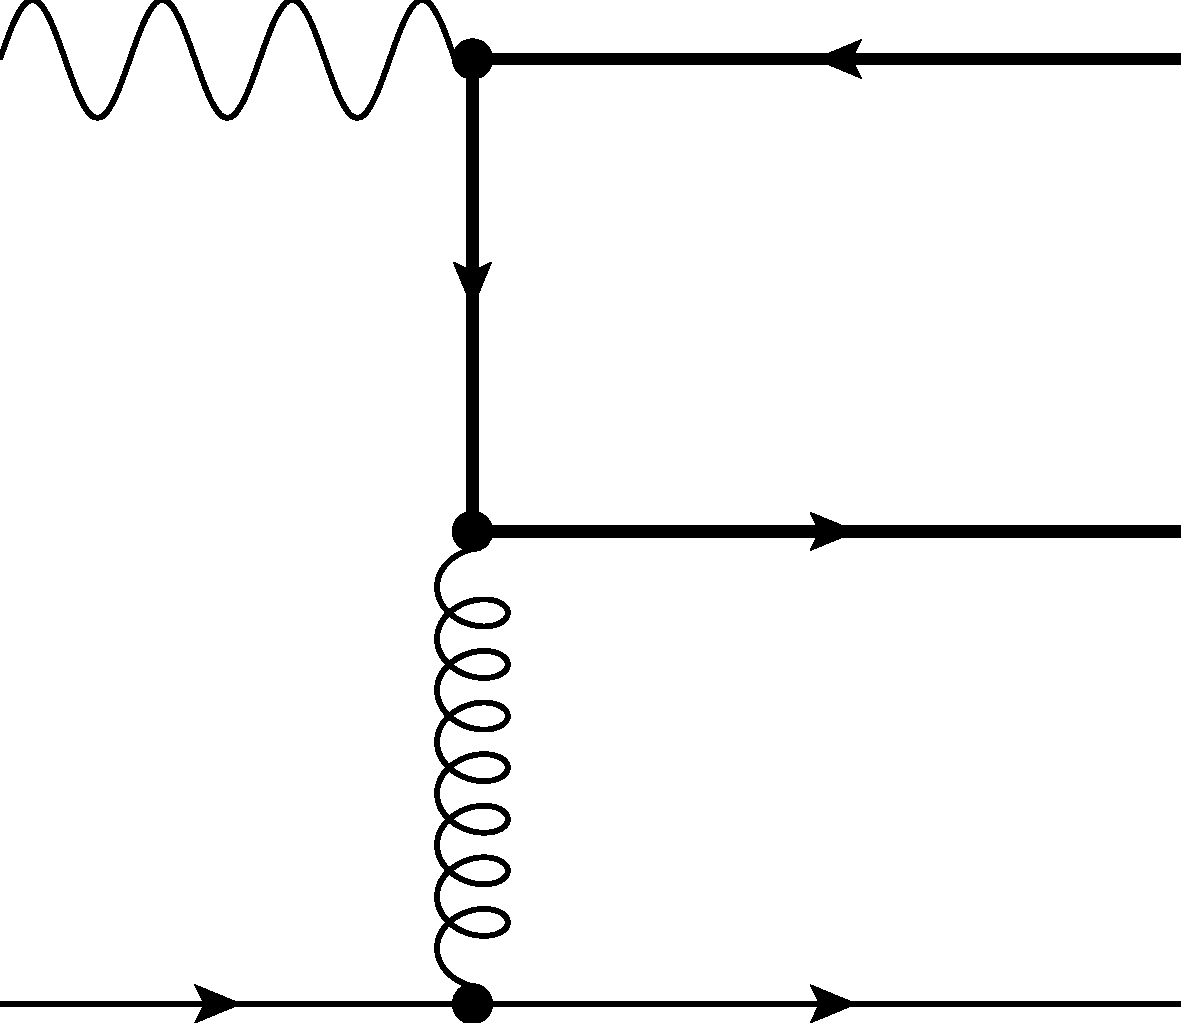
\includegraphics[width=\textwidth]{pyfeyn/nlo-q-1}
	\caption{}
\end{subfigure}\hspace{.02\textwidth}%
\begin{subfigure}[t]{.23\textwidth}
	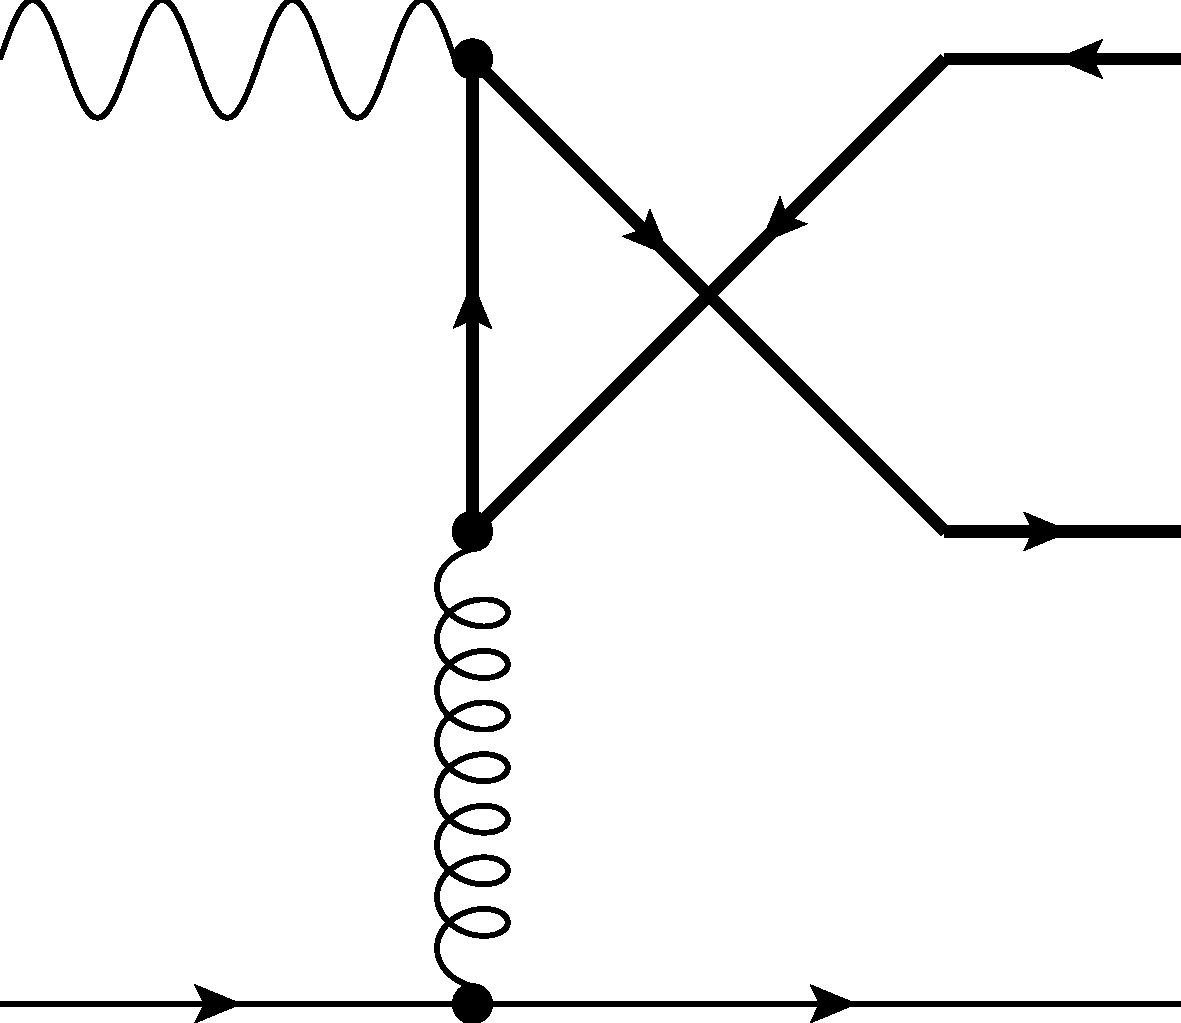
\includegraphics[width=\textwidth]{pyfeyn/nlo-q-2}
	\caption{}
\end{subfigure}\hspace{.02\textwidth}%
\begin{subfigure}[t]{.23\textwidth}
	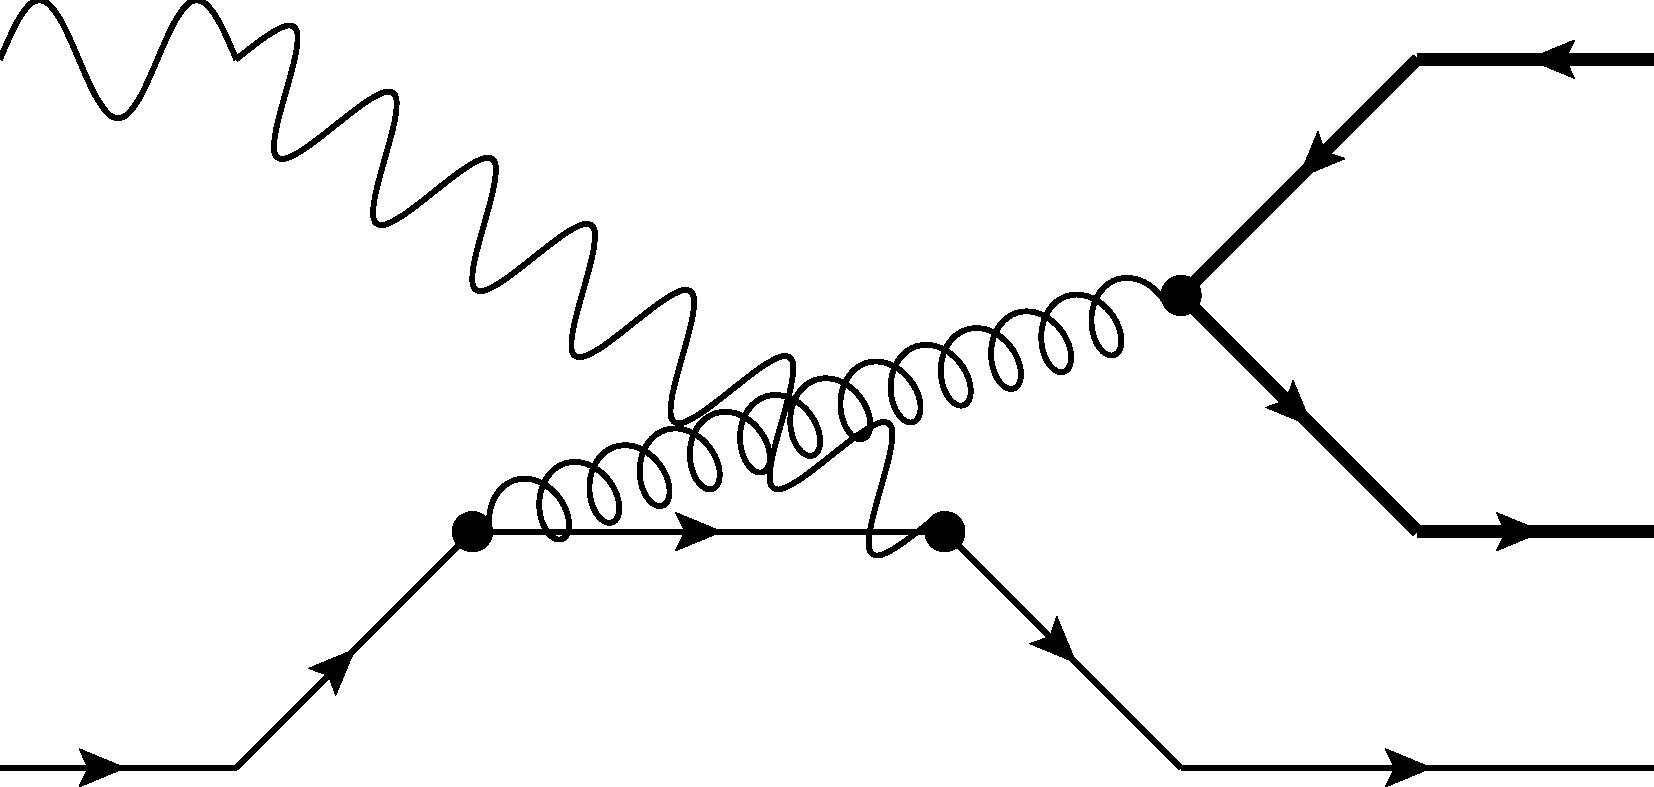
\includegraphics[width=\textwidth]{pyfeyn/nlo-q-3}
	\caption{}
\end{subfigure}\hspace{.02\textwidth}%
\begin{subfigure}[t]{.23\textwidth}
	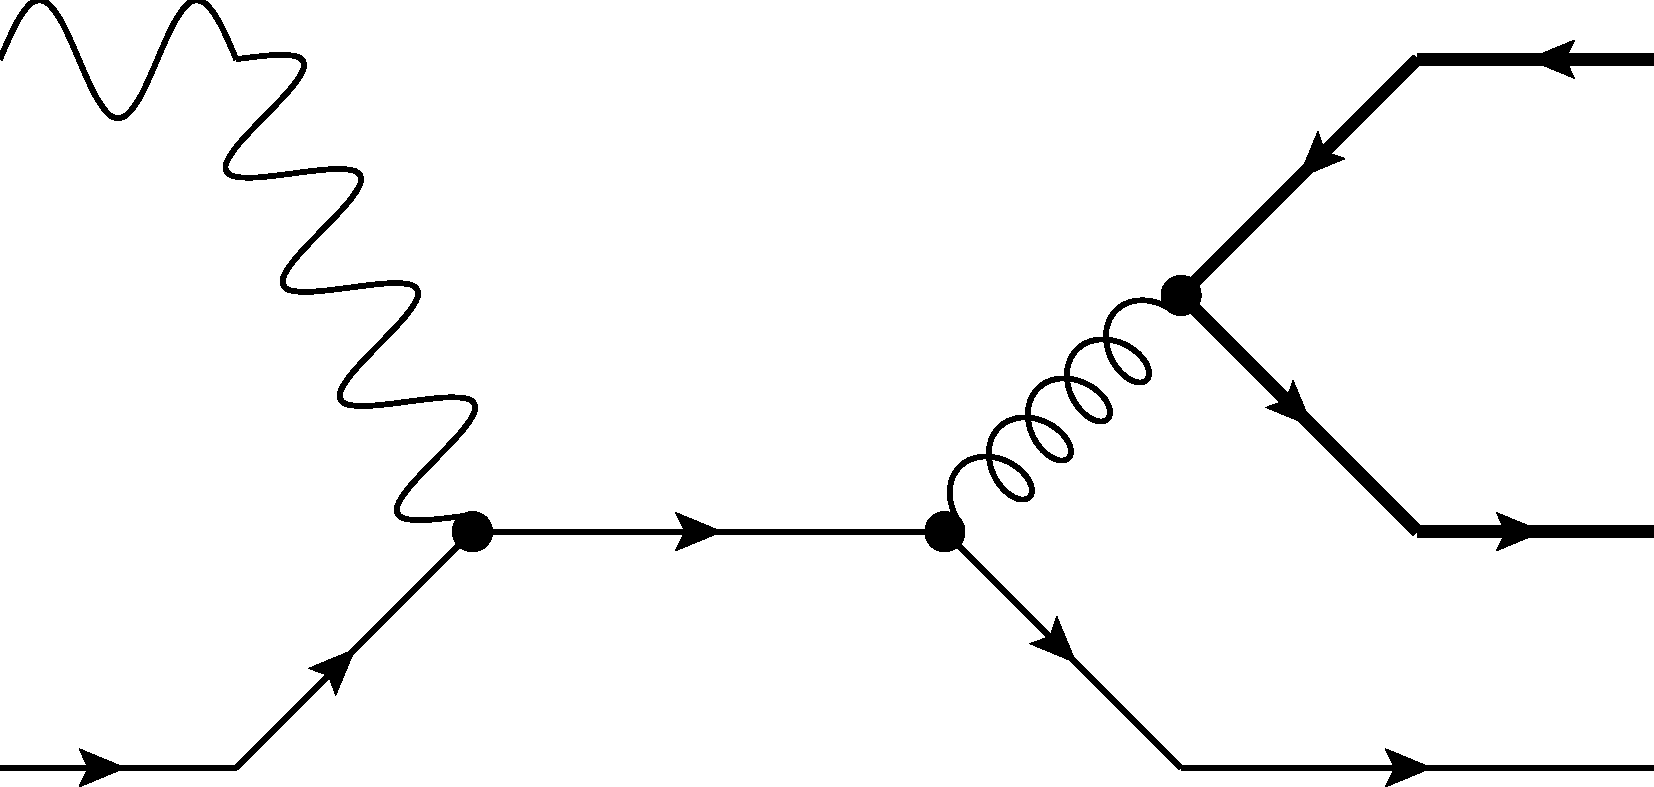
\includegraphics[width=\textwidth]{pyfeyn/nlo-q-4}
	\caption{}
\end{subfigure}
\caption{next-to-leading order Feynman diagrams for the light quark processes $i\varepsilon_{\Pgg}^\mu(q) u_{\Pq}^a(k_1)\Md^{(1),q}_{j,\mu a}$ }\label{fig:FeynNLOq}\fxerror{shift to appendix?}
\end{figure}

The result can then be written as
\begin{align}
M_k^{(1),\Pq} &=\hat {\mathcal P}_{k}^{\Pgg,\mu\mu'}\hat {\mathcal P}_{k}^{\Pq,aa'}\sum_{j,j'=1}^4\Md^{(1),q}_{j,\mu a}\left(\Md^{(1),q}_{j',\mu' a'}\right)^*\\
 &= 8g^4\mu_D^{-2\epsilon}e^2 N_C C_F\left( e_H^2 A_{k,1} +  e_L^2 A_{k,2} +  e_L e_H A_{k,3} \right)
\end{align}
where $e_L$ denotes the charge of the light quark $q$ in units of $e$.

For the light quark part we shift the occuring collinear ($y\rightarrow -1$) poles from the matrix elements to the phase space by dividing by $t'\propto(1+y)(1-x)$:
\begin{align}
dPS_{3,\Pq}' &= \frac{dPS_3}{t'} = dPS_3 \cdot \left(\frac {2s}{{s'}^2}\right)\frac 1 {(1-x)(1+y)}\\
 &= \frac {T_\epsilon}{\pi} \left(\frac {{s'}^2} s\right)^{\epsilon/2} (1-x)^{\epsilon}(1-y)^{\epsilon/2}(1+y)^{-1+\epsilon/2}dPS_2^{(5)}dy \sin^\epsilon(\theta_2)d\theta_2\\
{M_k^{(1),\Pq}}' &= t'M_k^{(1),\Pq}\\
\Rightarrow d\sigma_{k,\Pq}^{(1)} &= \frac{1}{2s'}\frac {K_{\Pq\Pgg}} 2 b_k(\epsilon) {M_k^{(1),\Pq}}' dPS_{3,\Pq}'
\end{align}

We can now use again the above defined distributions to replace the divergent factor $(1+y)^{-1+\epsilon/2}$ to split the light quark NLO part into two pieces\cite{Harris:1995tu}
\begin{align}
d\sigma_{k,\Pq}^{(1)} &= d\sigma_{k,\Pq}^{(1),c-} + d\sigma_{k,\Pq}^{(1),f}
\end{align}
corresponding to the collinear part ($d\sigma_{k,\Pq}^{(1),c-} \sim \delta(1+y)$) and the finite part ($d\sigma_{k,\Pq}^{(1),f}\sim\left(\frac 1 {1+y}\right)_\omega$). Note that for $q^2 < 0$ there is only a single collinear contribution ($y\rightarrow -1$) in $A_{k,1}$, i.e. $A_{k,2}$ does not contain any poles.

The results agree in the photo-production limit ($q^2\rightarrow 0$) with \cite{Bojak:1998zm}.
